
%% bare_jrnl.tex
%% V1.4
%% 2012/12/27
%% by Michael Shell
%% see http://www.michaelshell.org/
%% for current contact information.
%%
%% This is a skeleton file demonstrating the use of IEEEtran.cls
%% (requires IEEEtran.cls version 1.8 or later) with an IEEE journal paper.
%%
%% Support sites:
%% http://www.michaelshell.org/tex/ieeetran/
%% http://www.ctan.org/tex-archive/macros/latex/contrib/IEEEtran/
%% and
%% http://www.ieee.org/


\documentclass[journal]{IEEEtran}

\usepackage[utf8]{inputenc}
\usepackage[T1]{fontenc}
\usepackage{lmodern} % load a font with all the characters

\usepackage[style=numeric-comp,backend=biber,url=false]{biblatex}
\addbibresource{thesis-paper.bib}

\usepackage{cleveref}


% *** GRAPHICS RELATED PACKAGES ***
\usepackage[pdftex]{graphicx}
\graphicspath{{figures/}}
\DeclareGraphicsExtensions{.pdf,.jpg,.png}


% *** MATH PACKAGES ***
%
\usepackage[cmex10]{amsmath}
\interdisplaylinepenalty=2500

% correct bad hyphenation here
\hyphenation{}


\begin{document}
\boldmath

\title{Multi-purpose system for measuring electrical power supplied by electric sockets}

\author{Peter~Babič\\% <-this % stops a space
        Department of Theoretical and Industrial Electrical Engineering (DTIEE)\\%
        babicpet@gmail.com%
}

% The paper headers
\markboth{Paper covering Masters thesis, May~2016}%
{}


% make the title area
\maketitle


\begin{abstract}
This thesis shows the process of designing, building and programming of an inter-connected electronic system. It starts with explaining the fundamentals of the physics underlining the electronic power measurement process, transitioning into describing integrated components/modules used later in the proposed solution, such as ESP8266 Wi-Fi chip, GL.inet router board or OpenWRT - an unix-like operating system. The conceptual design of a final solution, utilising the aforementioned topics, follows. It includes diagrams describing the inner working of the hardware, and later software running on it. The manufactured device is capable of measuring the electric power provided by the electric socket to the appliance and send the measured values over Wi-Fi to the cloud, to be visualised on a custom web server employing a charting library to plot the measured quantities over time.
\end{abstract}

% Note that keywords are not normally used for peerreview papers.
\begin{IEEEkeywords}
electrical, power, socket, system
\end{IEEEkeywords}



\IEEEpeerreviewmaketitle



\section{Introduction}

\IEEEPARstart{T}{his} this paper is intended to sum up the research done in order to understand the Dynamics in electrical systems and their underlying differential equations.

 
\hfill June 03, 2015

\section{Dynamical Systems}
\textbf{Dynamical systems} are mathematical objects used to model physical phenomena whose state (or instantaneous description) changes over time \cite{katok1997introduction}. These models are used in financial and economic forecasting, environmental modeling, medical diagnosis, industrial equipment diagnosis, and a host of other applications.

For the most part, applications fall into three broad categories: predictive (also referred to as generative), in which the objective is to predict future states of the system from observations of the past and present states of the system, diagnostic, in which the objective is to infer what possible past states of the system might have led to the present state of the system (or observations leading up to the present state), and, finally, applications in which the objective is neither to predict the future nor explain the past but rather to provide a theory for the physical phenomena. These three categories correspond roughly to the need to predict, explain, and understand physical phenomena.

\subsection{Differential Equations}
A \textbf{differential equation} is any equation which contains derivatives, either ordinary derivatives or partial derivatives. Almost every physical situation that occurs in nature can be \textit{described} with an appropriate differential equation. 

The process of describing a physical situation with a differential equation is called \textbf{modeling}.

Differential equations are generally concerned about three questions:
\begin{enumerate}
\item Given a differential equation will a solution exist? 
\item If a differential equation does have a solution how many solutions are there?
\item If a differential equation does have a solution can we find it?
\end{enumerate}

The \textbf{order} or the differential equation is the highest derivative contained within it. \textbf{Degree} is the exponent on that highest derivative.

There are multiple ways to solve differential equations. From the numerical ones, notable are Euler's method and Runge-Kutta (RK4). Some other are described briefly in the following sections.

Differential equations fall to two groups - \textit{ordinary differential equations} (PDE) and \textit{partial differential equations}. Our study won't go into further detail about PDE and will stay focused mainly on ODE.


\subsection{Direction Field}
Understanding \textbf{direction fields} (or \textbf{slope fields)} and what they tell us about a differential equation and its solution is important and can be introduced without any knowledge of how to solve a differential equation and so can be done before the getting to actually solving them. 


The direction fields are important because they can provide a \textit{sketch of solution}, if exist, and a \textit{long term behavior} - most of the time we are interested in general picture about what is happening, as the time passes.

Example direction field, embedded in phase portrait is shown in \cref{f:vdp_m}.

\subsection{Laplace Transform}
The \textbf{Laplace transform} is an integral transform perhaps second only to the Fourier transform in its utility in solving physical problems. The Laplace transform \eqref{eq:lpl} is particularly useful in solving linear ordinary differential equations such as those arising in the analysis of electronic circuits. The Laplace transform $\mathcal{L}$
\begin{equation}
\label{eq:lpl} 
\mathcal{L}[f(t)](s)=\int{0}{\infty} f(t)e^{-st}dt
\end{equation}
where $f(t)$ is defined for $t\le 0$ - this is it's most common form and is called \textit{unilateral}.

Most important properties of Laplace transform is that differentiation and integration become multiplication and division. The transform turns integral equations and differential equations to polynomial equations, which are much easier to solve \cite{schiff2013laplace}. Once solved, use of the inverse Laplace transform reverts to the time domain.


\section{Periodic Orbits}
A periodic orbit corresponds to a special type of solution for a dynamical system, namely one which repeats itself in time. A dynamical system exhibiting a stable periodic orbit is often called an \textit{oscillator}. 

\subsection{Limit Cycle}
A \textbf{limit cycle} is an isolated closed trajectory. \textit{Isolated} means that neighboring trajectories are not closed - they spiral either towards or away from the limit cycle. The particle on the limit cycle, appears after one period on the exact same spot. Limit cycle appears on on a plane, opposed to a periodic orbit, that happens to be a vector.

%\begin{figure}[ht!]
%	\centering
%	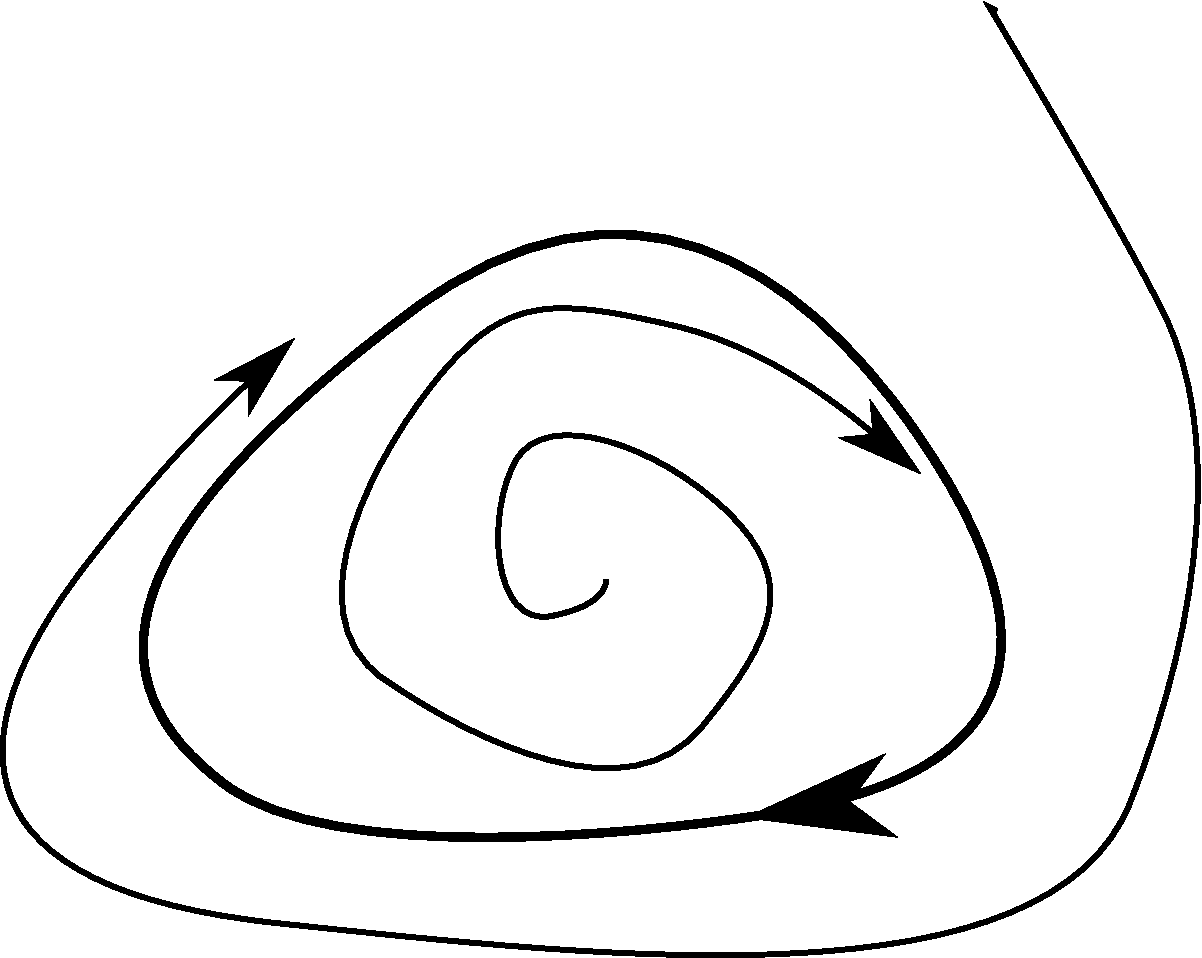
\includegraphics[width=.6\linewidth]{lcycle_stable}
%	\caption{Stable limit cycle. Trajectories spiral towards it.}
%	\label{f:lc_st}
%\end{figure}

If all neighboring trajectories approach the limit cycle, we say the limit cycle is \textbf{stable} or \textit{attracting}, as shown on \cref{f:lc_st}. Otherwise the limit cycle is \textbf{unstable}, or in exceptional cases, \textbf{half-stable}. Stable limit cycles are very important scientifically as they model systems that exhibit self-sustained oscillations. In other words, these systems oscillate even in the absence of external periodic forcing. 

%\begin{figure}[ht!]
%	\centering
%	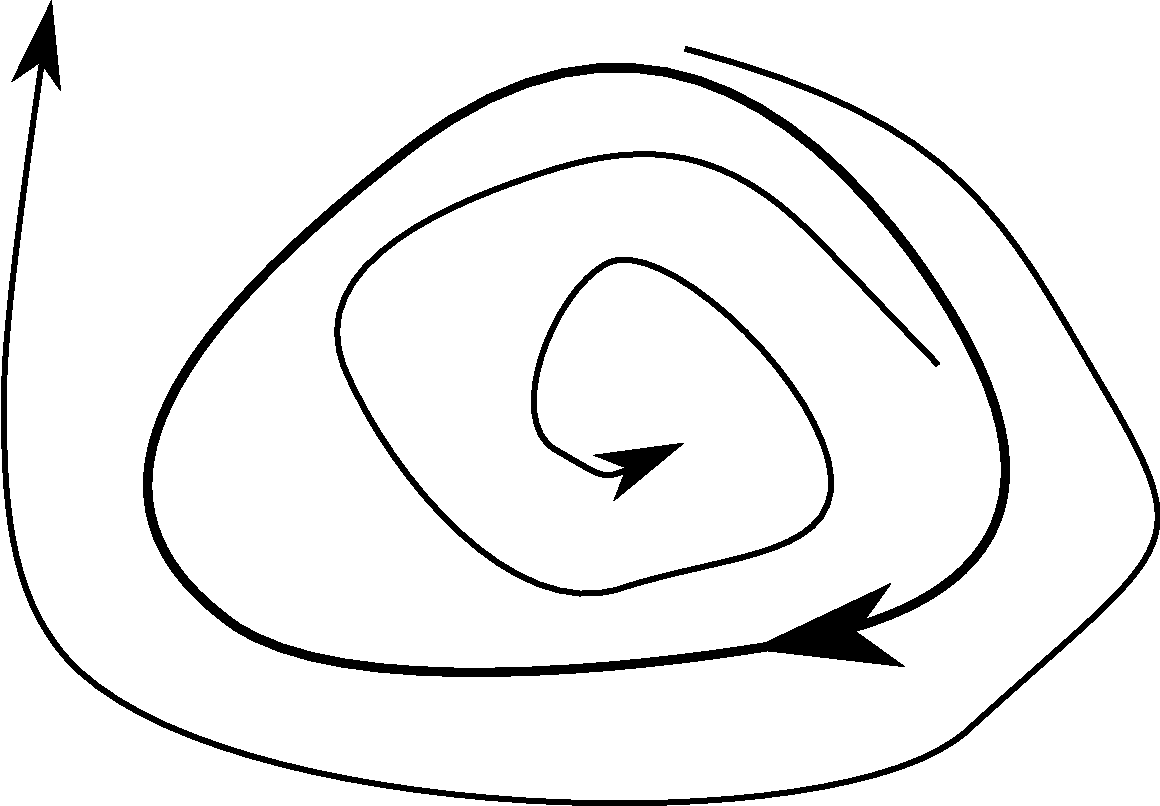
\includegraphics[width=.55\linewidth]{lcycle_unstable}
%	\caption{Unstable limit cycle. Trajectories spiral away from it.}
%	\label{f:lc_unst}
%\end{figure}

Of the countless examples that could be given, we mention only a few: the beating of a heart; the periodic ring of a pace maker neuron; daily rhythms in human body temperature and hormone secretion; chemical reactions that oscillate spontaneously; and dangerous self-excited vibrations in bridges and airplane wings. In each case, there is a standard oscillation of some preferred period, waveform, and amplitude. Oscillations are important part of electronics \cite{oscillations}, too.

If the system is perturbed slightly, it always returns to the standard cycle. Limit cycles are inherently nonlinear phenomena; they cant occur in linear systems \cite{strogatz2008nonlinear}.

%\begin{figure}[ht!]
%	\centering
%	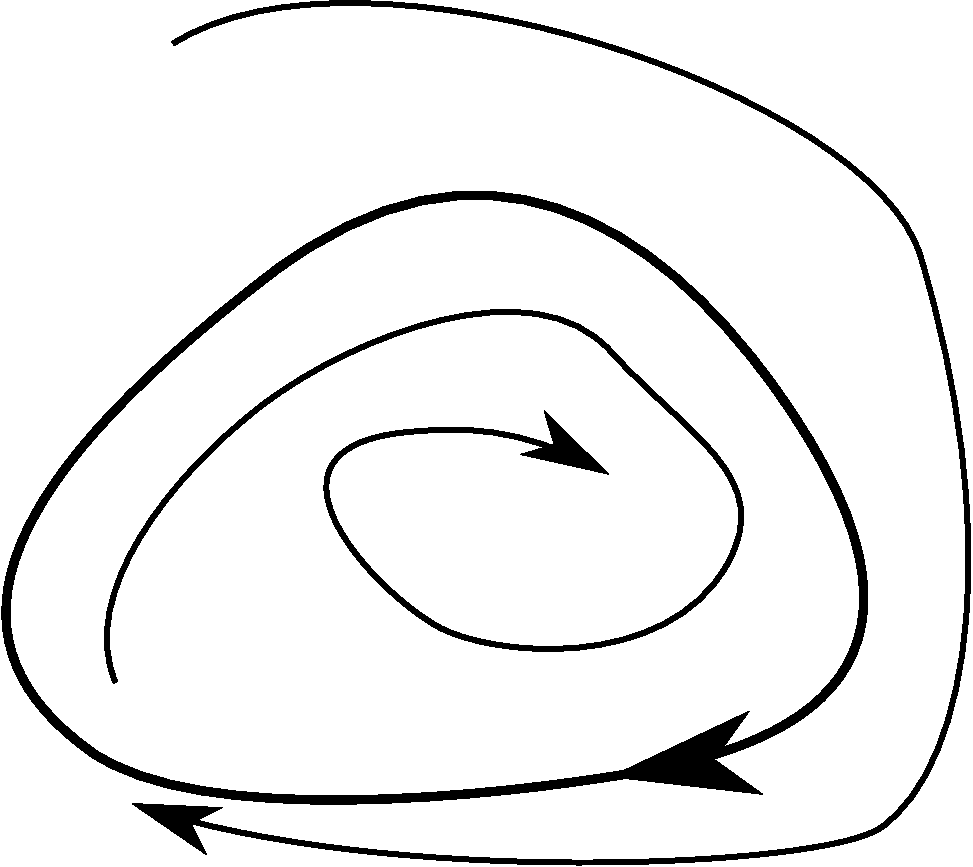
\includegraphics[width=.5\linewidth]{lcycle_hstable}
%	\caption{Half-stable (or semi-stable) limit cycle. Attract trajectories from one side and repel them from other side.}
%	\label{f:lc_hst}
%\end{figure}

\subsection{Damping}
Mentioning damping is important mainly because, in a real world, oscillations eventually stop, due to Newton's law of Thermodynamics (the frictional force). In electronics, there is no ideal oscillator, too - small amount of energy is lost every cycle, due to electric resistance.

Generally, the damping is linear either linear or nonlinear. As a rule of thumb, the linear one is easily modeled mathematically, obeying known rules, while the nonlinear one is not \cite{institute1989estimation}. Nonlinear damping is advantageous in multiple cases and the research is still ongoing about this topic.

There are four exclusive states, that damping in a system can be in:
\begin{enumerate}
\item Undamped
\item Underdumped
\item Critically-dumped
\item Overdumped
\end{enumerate}

\section{Advanced Studies}

\subsection{Li\'{e}nard Equation}
A nonlinear second-order ordinary differential equation
\begin{equation}
\label{eq:lnrd}
y''+f(x)x'+x=0
\end{equation}

This equation describes the dynamics of a system with one degree of freedom in the presence of a linear restoring force and nonlinear damping. The function $f$ has properties
\begin{align*}
f(x)&<0\quad for\,small\,|x| \\
f(x)&>0\quad for\,large\,|x|
\end{align*}
that is, if for small amplitudes the system absorbs energy and for large amplitudes dissipation occurs, then in the system one can expect self-exciting oscillations.

\textbf{Li\'{e}nard equation} was intensely studied as it can be used to model oscillating circuits. Under certain additional assumptions Li\'{e}nard's theorem guarantees the uniqueness and existence of a limit cycle for such a system.

\subsection{Van der Pol Equation}
One of the most well-known oscillator model in dynamics is \textbf{Van der Pol oscillator}, which is a special case of Li\'{e}nard's equation \eqref{eq:lnrd} and is described by a differential equation
\begin{equation}
\label{eq:vdp}
y''-\mu\left(1-y^2\right)y'+y=0
\end{equation}
where $y$ is the dynamical variable and $\mu>0$ is a parameter. If $\mu=0$, then the equation reduces to the equation of simple harmonic motion
$$y''+y=0$$
The $\mu$ parameter determines the shape of the limit cycle. As it approaches 0, it gets the shape of a circle. On the other hand, increasing the paramter, involves sharpening of the curves.

The Van der Pol equation \eqref{eq:vdp} arises in the study of circuits containing vacuum tubes (triode) and is derived from earlier, Rayleigh equation \cite{nahin2001science}, known also as Rayleigh-Plesset equation - an ordinary differential equation explaining the dynamics of a spherical bubble in an infinite body of liquid.

Van der Pol oscillator is \textbf{self-sustainable}, \textbf{relaxation} oscillator. Self-sustainability in this context means, that the energy is fed into small oscillations and removed from large oscillations. Relaxation means, that the energy is gradually accumulating over time and then quickly released (relaxed). In electronics jargon, the relaxation oscillator is also called a \textit{free-running} oscillator. As already explained, it does not require neither one (monostable), nor two (bistable) inputs for transitioning between states, it "runs" by itself, thus free-running.

\subsection{Periodicity in Van der Pol's Oscillator}
Li\'{e}nard's theorem can be used to prove that the system described by  Van der Pol equation \eqref{eq:vdp} has a limit cycle \cite{sternberg2014dynamical}. If we want to visualize it, the one-dimensional form of equation must be first \textit{transformed} to the two-dimensional form. Applying the Li\'{e}nard transformation $$y=x-\frac{x^3}{3}-\frac{\dot x}{\mu}$$ where dot indicates the time derivative, the system can be written in it's two-dimensional form \cite{kaplan2012understanding}:
\begin{align*}
\dot x &= \mu \left(x-\frac13 x^3 -y\right) \\
\dot y &= \frac{1}{\mu} x
\end{align*}

However, this form is not well-known. Far common form uses the transformation $y=\dot x$, that yields
\begin{align*}
\dot x &= y \\
\dot y &= \mu\left(1-x^2\right)y-x
\end{align*}
which can be plotted onto direction field, as shown on \cref{f:vdp_m}. It is possible to see the stable limit cycle as well as trajectories from both sides attracted towards it.

The Van der Pol oscillator can be forced too, however, this work does not aim to investigate further in this direction.

%\begin{figure}[ht!]
%	\centering
%	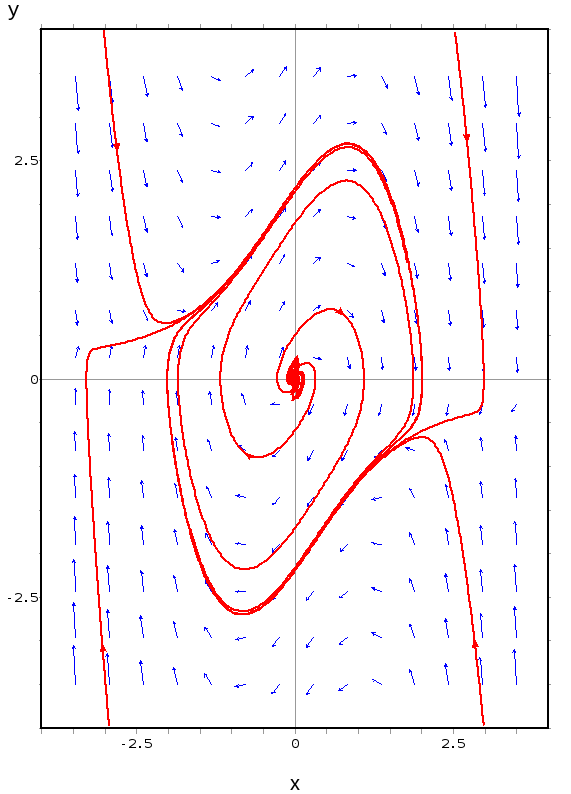
\includegraphics[width=.85\linewidth]{vdp_maxima}
%	\caption{Phase portrait of the unforced Van der Pol oscillator, showing a limit cycle and the direction field Parameter $\mu=1$. The wxMaxima computing software was used for this purpose. }
%	\label{f:vdp_m}
%\end{figure}

\subsection{Josephson Junctions}
Another phenomenon regarding nonlinear dynamics applied in the field of electrical engineering is known as Josephson Junction.

\textbf{Josephson junctions} are superconducting devices that are capable of generating voltage oscillations of extraordinary high frequency, typically 10\textsuperscript{10} - 10\textsuperscript{11} cycles per second \cite{van1981principles}. They consist of two superconducting layers, separated by a very thin insulator that weakly couples them, as shown on \cref{f:jjunc}.

%\begin{figure}[ht!]
%	\centering
%	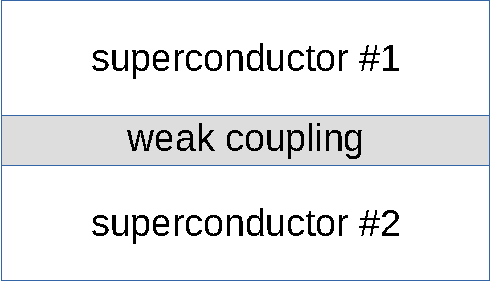
\includegraphics[width=.4\linewidth]{jjunc}
%	\caption{The physical structure of a Josephson Junction. Shown for ilustration purposes.}
%	\label{f:jjunc}
%\end{figure}

Although quantum mechanics is required to explain the origin of the Josephson effect, we can nevertheless dive into dynamics of Josephson junctions in classical terms. They have been particularly useful for \textit{experimental} studies of nonlinear dynamics, because the equation governing a single junction resembles the one of a pendulum \cite{strogatz1994nonlinear}.

Josephson junctions are used to detect extremely low electric potentials and are used for instance, to detect far-infrared radiation from distant galaxies. They are also formed to arrays, because there is a great potential seen in this configuration, however, all the effects are yet to be fully understood.

\subsection{Applications in Electrical Circuits}
This is the main section of our work. We will investigate, what is the behavior of electrical components in circuits with respect to time and model them with differential equations.

\textbf{Resistor} is a linear component. It is described by an \textbf{Ohm's law}, which states, that the voltage $V$ across it is proportional to the current $I$ passing through it's resistance $R$.
$$V=IR$$

\textbf{Inductor} is one nonlinear component. It produces a voltage drop, that is proportional to the \textit{rate of change} of the current through it, as described by \textbf{Faraday's Law}
$$V(t)=L\,\frac{dI}{dt}$$

\textbf{Capacitor} is another nonlinear component. Voltage drop across it, is on the other hand proportional to the charge stored in it. This behavior is derived from  \textbf{Coulumb's law}
$$V(t)=\frac{1}{C}\int i\,dt$$

\textbf{Kirchhoff Current Law} (KCL) states, that the algebraic sum of the currents flowing into any junction of an electric circuit must be zero.

\textbf{Kirchhoff Voltage Law} (KVL) states, that the algebraic sum of the voltage drops around any closed loop in an electric circuit must be zero.

These laws allow us to model, what is happening inside the circuit with respect to time \cite{lynch2013dynamical}.

\section{First-order Electrical Circuits}
First order circuits generally contain one energy-storing (nonlinear) element.

\subsection{RL Circuit}
The RL circuit shown on \cref{f:rl} has a resistor and an inductor connected in series. A \textit{constant} voltage $V$ is applied when the switch is closed.

%\begin{figure}[ht!]
%	\centering
%	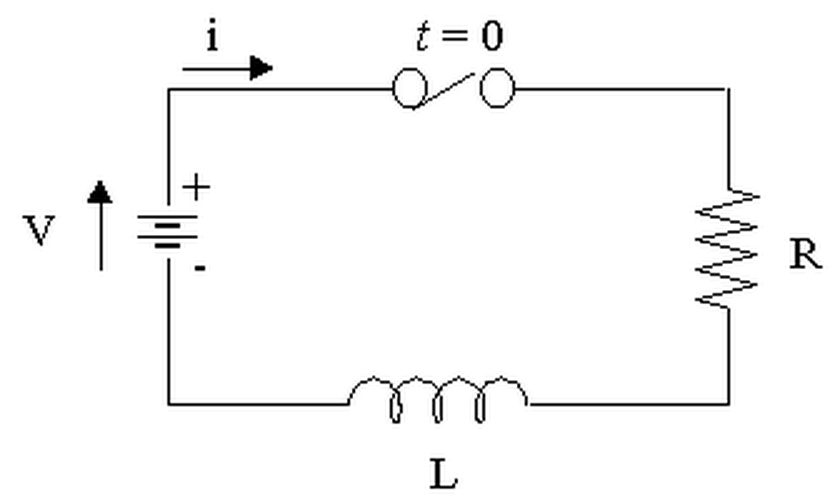
\includegraphics[width=.75\linewidth]{rl}
%	\caption{RL circuit diagram.}
%	\label{f:rl}
%\end{figure}

Applying the KVL, we obtain the algebraic sums of all the voltage drops as an ODE with respect to time
$$Ri+L\,\frac{di}{dt}=V(t)$$
solving which we obtain 
$$i=\frac{V}{R}\left(1-e^{-(R/L)t}\right)$$
The solving process is quite lenghty and is not a point of this work. For more details see \cite{bird2014electrical}.

If the applied voltage is not constant, but rather \textit{variable}, in the form of $V(t)=A\,cos(\omega(t) + \phi)$ or $V(t)=A\,sin(\omega(t) + \phi)$, then things get complex.

\subsection{RC Circuits}
The RC circuit shown on \cref{f:rc} has a resistor and unexpectedly, a capacitor connected in series. Again, A \textit{constant} voltage $V$ is applied when the switch is closed.

%\begin{figure}[ht!]
%	\centering
%	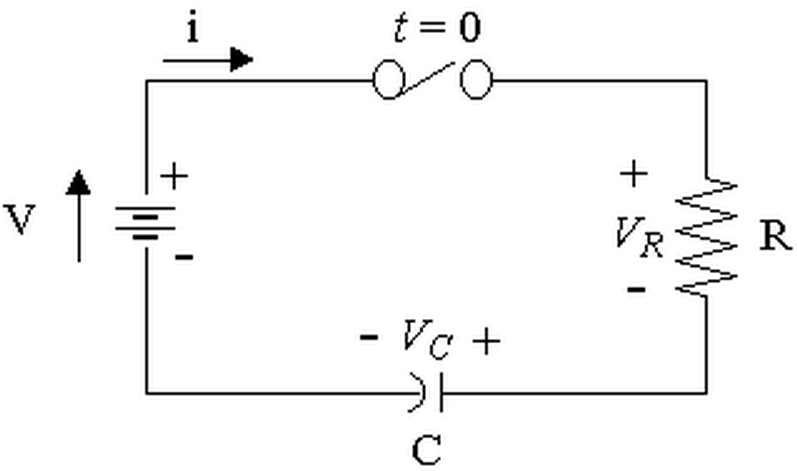
\includegraphics[width=.75\linewidth]{rc}
%	\caption{RC circuit diagram.}
%	\label{f:rc}
%\end{figure}

Kirchhoff's voltage law says the total voltages must be zero. So applying this law to a series RC circuit results in the equation
$$Ri+\frac{1}{C}\int i\,dt=V(t)$$
Again, to solve it, we can turn it into a differential equation, by differentiating throughout with respect to $t$
$$R\,\frac{di}{dt}+\frac{i}{C}=0$$
solving which we obtain
$$i=\frac{V}{R}\,e^{-t/RC}$$





\section{Second-order Electrical Circuits}
Second order circuits contain both nonlinear elements. A RLC circuit consist of the resistor, the inductor and the capacitor and is shown in \cref{f:rlc}.

%\begin{figure}[ht!]
%	\centering
%	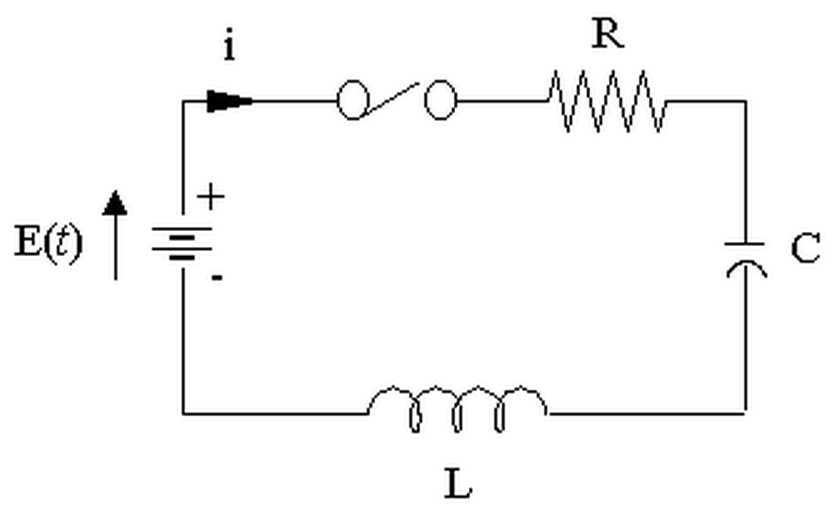
\includegraphics[width=.75\linewidth]{rlc}
%	\caption{RLC circuit diagram.}
%	\label{f:rlc}
%\end{figure}

In order to follow further, we must define new term, that will be used. \textbf{Electro-motive force} (EMF) is the force, that moves electrons from lower potential to the higher one, as opposed to so far mentioned electric potential, that can do it only in reverse order. The source of EMF can be for instance chemical reaction in cell battery, that induces the \textit{separation of charge}.

The EMF is mentioned, because nonlinear elements (capacitor and inductor) store and release energy, as well as cells do. Thus they have the ability to move electrons from one potential to another and so they have to be described in terms of electro-magnetic force, instead of just electric potential.

If the driving force in RLC circuit is \textbf{constant}, the current equation for a circuit is
$$L\,\frac{di}{dt} + Ri + \frac{1}{C}\int i\,dt = E$$
Differentiating we obtain
$$L\,\frac{d^2i}{dt^2} + R\,\frac{di}{dt} + \frac1C\,i = 0$$
which is the second order linear differential equation (homogenous).

The circuit itself is a damped oscillator. Writing the equation in its auxiliary form and finding its roots, we could obtain a formula for it's \textit{damping factor}, however, it is a topic far off the boundaries of this work.

If the non-constant (variable) driving force, the things get even more complicated. For instance, Laplace transform can be used to solve the equations.

\section{Conclusion}
We have dived into multiple mathematical theories and science fields that has some connection to dynamical systems and electrical circuits. The topics mentioned are only scratch on the surface. Every single one could be written in separate paper or even a book. In fact, thousands of book have been written in mentioned topics and there are probably thousands more to come.

There are multiple important topics, namely \textit{bifurcations} and \textit{chaos}, but we decided to skip them, because of the vast amount of information, they represent and also due to lack of direct connection between them and electical circuits.

The main goal was to get some general idea about the connections between the terms and get some picture of the problematic. Although probably in a chaotic way, that goal was met and we tried to be as concise as possible along the way.


% if have a single appendix:
%\appendix[Proof of the Zonklar Equations]
% or
%\appendix  % for no appendix heading
% do not use \section anymore after \appendix, only \section*
% is possibly needed

% use appendices with more than one appendix
% then use \section to start each appendix
% you must declare a \section before using any
% \subsection or using \label (\appendices by itself
% starts a section numbered zero.)
%


%\appendices
%\section{Proof of the First Zonklar Equation}
%Appendix one text goes here. 
%
%% you can choose not to have a title for an appendix
%% if you want by leaving the argument blank
%\section{}
%Appendix two text goes here.


% use section* for acknowledgement
\section*{Acknowledgment}
The authors would like to thank professor Carlos Par\'{e}s for having patience with them. Another thank would go to the well-written book \emph{Nonlinear Dynamics and Chaos, S.H. Strogatz, 2008} for introduction to and for sparking curiosity in the field of Dynamical Systems.

% Can use something like this to put references on a page
% by themselves when using endfloat and the captionsoff option.
%\ifCLASSOPTIONcaptionsoff
  \newpage
%\fi

\printbibliography



% that's all folks
\end{document}





% An example of a floating figure using the graphicx package.
% Note that \label must occur AFTER (or within) \caption.
% For figures, \caption should occur after the \includegraphics.
% Note that IEEEtran v1.7 and later has special internal code that
% is designed to preserve the operation of \label within \caption
% even when the captionsoff option is in effect. However, because
% of issues like this, it may be the safest practice to put all your
% \label just after \caption rather than within \caption{}.
%
% Reminder: the "draftcls" or "draftclsnofoot", not "draft", class
% option should be used if it is desired that the figures are to be
% displayed while in draft mode.
%
%\begin{figure}[!t]
%\centering
%\includegraphics[width=2.5in]{myfigure}
% where an .eps filename suffix will be assumed under latex, 
% and a .pdf suffix will be assumed for pdflatex; or what has been declared
% via \DeclareGraphicsExtensions.
%\caption{Simulation Results.}
%\label{fig_sim}
%\end{figure}

% Note that IEEE typically puts floats only at the top, even when this
% results in a large percentage of a column being occupied by floats.


% An example of a double column floating figure using two subfigures.
% (The subfig.sty package must be loaded for this to work.)
% The subfigure \label commands are set within each subfloat command,
% and the \label for the overall figure must come after \caption.
% \hfil is used as a separator to get equal spacing.
% Watch out that the combined width of all the subfigures on a 
% line do not exceed the text width or a line break will occur.
%
%\begin{figure*}[!t]
%\centering
%\subfloat[Case I]{\includegraphics[width=2.5in]{box}%
%\label{fig_first_case}}
%\hfil
%\subfloat[Case II]{\includegraphics[width=2.5in]{box}%
%\label{fig_second_case}}
%\caption{Simulation results.}
%\label{fig_sim}
%\end{figure*}
%
% Note that often IEEE papers with subfigures do not employ subfigure
% captions (using the optional argument to \subfloat[]), but instead will
% reference/describe all of them (a), (b), etc., within the main caption.


% An example of a floating table. Note that, for IEEE style tables, the 
% \caption command should come BEFORE the table. Table text will default to
% \footnotesize as IEEE normally uses this smaller font for tables.
% The \label must come after \caption as always.
%
%\begin{table}[!t]
%% increase table row spacing, adjust to taste
%\renewcommand{\arraystretch}{1.3}
% if using array.sty, it might be a good idea to tweak the value of
% \extrarowheight as needed to properly center the text within the cells
%\caption{An Example of a Table}
%\label{table_example}
%\centering
%% Some packages, such as MDW tools, offer better commands for making tables
%% than the plain LaTeX2e tabular which is used here.
%\begin{tabular}{|c||c|}
%\hline
%One & Two\\
%\hline
%Three & Four\\
%\hline
%\end{tabular}
%\end{table}


% Note that IEEE does not put floats in the very first column - or typically
% anywhere on the first page for that matter. Also, in-text middle ("here")
% positioning is not used. Most IEEE journals use top floats exclusively.
% Note that, LaTeX2e, unlike IEEE journals, places footnotes above bottom
% floats. This can be corrected via the \fnbelowfloat command of the
% stfloats package.




% Some very useful LaTeX packages include:
% (uncomment the ones you want to load)


% *** MISC UTILITY PACKAGES ***
%
%\usepackage{ifpdf}
% Heiko Oberdiek's ifpdf.sty is very useful if you need conditional
% compilation based on whether the output is pdf or dvi.
% usage:
% \ifpdf
%   % pdf code
% \else
%   % dvi code
% \fi
% The latest version of ifpdf.sty can be obtained from:
% http://www.ctan.org/tex-archive/macros/latex/contrib/oberdiek/
% Also, note that IEEEtran.cls V1.7 and later provides a builtin
% \ifCLASSINFOpdf conditional that works the same way.
% When switching from latex to pdflatex and vice-versa, the compiler may
% have to be run twice to clear warning/error messages.






% *** CITATION PACKAGES ***
%
%\usepackage{cite}
% cite.sty was written by Donald Arseneau
% V1.6 and later of IEEEtran pre-defines the format of the cite.sty package
% \cite{} output to follow that of IEEE. Loading the cite package will
% result in citation numbers being automatically sorted and properly
% "compressed/ranged". e.g., [1], [9], [2], [7], [5], [6] without using
% cite.sty will become [1], [2], [5]--[7], [9] using cite.sty. cite.sty's
% \cite will automatically add leading space, if needed. Use cite.sty's
% noadjust option (cite.sty V3.8 and later) if you want to turn this off
% such as if a citation ever needs to be enclosed in parenthesis.
% cite.sty is already installed on most LaTeX systems. Be sure and use
% version 4.0 (2003-05-27) and later if using hyperref.sty. cite.sty does
% not currently provide for hyperlinked citations.
% The latest version can be obtained at:
% http://www.ctan.org/tex-archive/macros/latex/contrib/cite/
% The documentation is contained in the cite.sty file itself.






% *** MATH PACKAGES ***
%
%\usepackage[cmex10]{amsmath}
% A popular package from the American Mathematical Society that provides
% many useful and powerful commands for dealing with mathematics. If using
% it, be sure to load this package with the cmex10 option to ensure that
% only type 1 fonts will utilized at all point sizes. Without this option,
% it is possible that some math symbols, particularly those within
% footnotes, will be rendered in bitmap form which will result in a
% document that can not be IEEE Xplore compliant!
%
% Also, note that the amsmath package sets \interdisplaylinepenalty to 10000
% thus preventing page breaks from occurring within multiline equations. Use:
%\interdisplaylinepenalty=2500
% after loading amsmath to restore such page breaks as IEEEtran.cls normally
% does. amsmath.sty is already installed on most LaTeX systems. The latest
% version and documentation can be obtained at:
% http://www.ctan.org/tex-archive/macros/latex/required/amslatex/math/





% *** SPECIALIZED LIST PACKAGES ***
%
%\usepackage{algorithmic}
% algorithmic.sty was written by Peter Williams and Rogerio Brito.
% This package provides an algorithmic environment fo describing algorithms.
% You can use the algorithmic environment in-text or within a figure
% environment to provide for a floating algorithm. Do NOT use the algorithm
% floating environment provided by algorithm.sty (by the same authors) or
% algorithm2e.sty (by Christophe Fiorio) as IEEE does not use dedicated
% algorithm float types and packages that provide these will not provide
% correct IEEE style captions. The latest version and documentation of
% algorithmic.sty can be obtained at:
% http://www.ctan.org/tex-archive/macros/latex/contrib/algorithms/
% There is also a support site at:
% http://algorithms.berlios.de/index.html
% Also of interest may be the (relatively newer and more customizable)
% algorithmicx.sty package by Szasz Janos:
% http://www.ctan.org/tex-archive/macros/latex/contrib/algorithmicx/




% *** ALIGNMENT PACKAGES ***
%
%\usepackage{array}
% Frank Mittelbach's and David Carlisle's array.sty patches and improves
% the standard LaTeX2e array and tabular environments to provide better
% appearance and additional user controls. As the default LaTeX2e table
% generation code is lacking to the point of almost being broken with
% respect to the quality of the end results, all users are strongly
% advised to use an enhanced (at the very least that provided by array.sty)
% set of table tools. array.sty is already installed on most systems. The
% latest version and documentation can be obtained at:
% http://www.ctan.org/tex-archive/macros/latex/required/tools/


% IEEEtran contains the IEEEeqnarray family of commands that can be used to
% generate multiline equations as well as matrices, tables, etc., of high
% quality.




% *** SUBFIGURE PACKAGES ***
%\ifCLASSOPTIONcompsoc
%  \usepackage[caption=false,font=normalsize,labelfont=sf,textfont=sf]{subfig}
%\else
%  \usepackage[caption=false,font=footnotesize]{subfig}
%\fi
% subfig.sty, written by Steven Douglas Cochran, is the modern replacement
% for subfigure.sty, the latter of which is no longer maintained and is
% incompatible with some LaTeX packages including fixltx2e. However,
% subfig.sty requires and automatically loads Axel Sommerfeldt's caption.sty
% which will override IEEEtran.cls' handling of captions and this will result
% in non-IEEE style figure/table captions. To prevent this problem, be sure
% and invoke subfig.sty's "caption=false" package option (available since
% subfig.sty version 1.3, 2005/06/28) as this is will preserve IEEEtran.cls
% handling of captions.
% Note that the Computer Society format requires a larger sans serif font
% than the serif footnote size font used in traditional IEEE formatting
% and thus the need to invoke different subfig.sty package options depending
% on whether compsoc mode has been enabled.
%
% The latest version and documentation of subfig.sty can be obtained at:
% http://www.ctan.org/tex-archive/macros/latex/contrib/subfig/




% *** FLOAT PACKAGES ***
%
%\usepackage{fixltx2e}
% fixltx2e, the successor to the earlier fix2col.sty, was written by
% Frank Mittelbach and David Carlisle. This package corrects a few problems
% in the LaTeX2e kernel, the most notable of which is that in current
% LaTeX2e releases, the ordering of single and double column floats is not
% guaranteed to be preserved. Thus, an unpatched LaTeX2e can allow a
% single column figure to be placed prior to an earlier double column
% figure. The latest version and documentation can be found at:
% http://www.ctan.org/tex-archive/macros/latex/base/


%\usepackage{stfloats}
% stfloats.sty was written by Sigitas Tolusis. This package gives LaTeX2e
% the ability to do double column floats at the bottom of the page as well
% as the top. (e.g., "\begin{figure*}[!b]" is not normally possible in
% LaTeX2e). It also provides a command:
%\fnbelowfloat
% to enable the placement of footnotes below bottom floats (the standard
% LaTeX2e kernel puts them above bottom floats). This is an invasive package
% which rewrites many portions of the LaTeX2e float routines. It may not work
% with other packages that modify the LaTeX2e float routines. The latest
% version and documentation can be obtained at:
% http://www.ctan.org/tex-archive/macros/latex/contrib/sttools/
% Do not use the stfloats baselinefloat ability as IEEE does not allow
% \baselineskip to stretch. Authors submitting work to the IEEE should note
% that IEEE rarely uses double column equations and that authors should try
% to avoid such use. Do not be tempted to use the cuted.sty or midfloat.sty
% packages (also by Sigitas Tolusis) as IEEE does not format its papers in
% such ways.
% Do not attempt to use stfloats with fixltx2e as they are incompatible.
% Instead, use Morten Hogholm'a dblfloatfix which combines the features
% of both fixltx2e and stfloats:
%
% \usepackage{dblfloatfix}
% The latest version can be found at:
% http://www.ctan.org/tex-archive/macros/latex/contrib/dblfloatfix/




%\ifCLASSOPTIONcaptionsoff
%  \usepackage[nomarkers]{endfloat}
% \let\MYoriglatexcaption\caption
% \renewcommand{\caption}[2][\relax]{\MYoriglatexcaption[#2]{#2}}
%\fi
% endfloat.sty was written by James Darrell McCauley, Jeff Goldberg and 
% Axel Sommerfeldt. This package may be useful when used in conjunction with 
% IEEEtran.cls'  captionsoff option. Some IEEE journals/societies require that
% submissions have lists of figures/tables at the end of the paper and that
% figures/tables without any captions are placed on a page by themselves at
% the end of the document. If needed, the draftcls IEEEtran class option or
% \CLASSINPUTbaselinestretch interface can be used to increase the line
% spacing as well. Be sure and use the nomarkers option of endfloat to
% prevent endfloat from "marking" where the figures would have been placed
% in the text. The two hack lines of code above are a slight modification of
% that suggested by in the endfloat docs (section 8.4.1) to ensure that
% the full captions always appear in the list of figures/tables - even if
% the user used the short optional argument of \caption[]{}.
% IEEE papers do not typically make use of \caption[]'s optional argument,
% so this should not be an issue. A similar trick can be used to disable
% captions of packages such as subfig.sty that lack options to turn off
% the subcaptions:
% For subfig.sty:
% \let\MYorigsubfloat\subfloat
% \renewcommand{\subfloat}[2][\relax]{\MYorigsubfloat[]{#2}}
% However, the above trick will not work if both optional arguments of
% the \subfloat command are used. Furthermore, there needs to be a
% description of each subfigure *somewhere* and endfloat does not add
% subfigure captions to its list of figures. Thus, the best approach is to
% avoid the use of subfigure captions (many IEEE journals avoid them anyway)
% and instead reference/explain all the subfigures within the main caption.
% The latest version of endfloat.sty and its documentation can obtained at:
% http://www.ctan.org/tex-archive/macros/latex/contrib/endfloat/
%
% The IEEEtran \ifCLASSOPTIONcaptionsoff conditional can also be used
% later in the document, say, to conditionally put the References on a 
% page by themselves.




% *** PDF, URL AND HYPERLINK PACKAGES ***
%
%\usepackage{url}
% url.sty was written by Donald Arseneau. It provides better support for
% handling and breaking URLs. url.sty is already installed on most LaTeX
% systems. The latest version and documentation can be obtained at:
% http://www.ctan.org/tex-archive/macros/latex/contrib/url/
% Basically, \url{my_url_here}.







% trigger a \newpage just before the given reference
% number - used to balance the columns on the last page
% adjust value as needed - may need to be readjusted if
% the document is modified later
%\IEEEtriggeratref{8}
% The "triggered" command can be changed if desired:
%\IEEEtriggercmd{\enlargethispage{-5in}}

% references section

% can use a bibliography generated by BibTeX as a .bbl file
% BibTeX documentation can be easily obtained at:
% http://www.ctan.org/tex-archive/biblio/bibtex/contrib/doc/
% The IEEEtran BibTeX style support page is at:
% http://www.michaelshell.org/tex/ieeetran/bibtex/
% argument is your BibTeX string definitions and bibliography database(s)
%\bibliographystyle{IEEEtran}
%\bibliography{IEEEabrv,electrical}
%\pagebreak

% <OR> manually copy in the resultant .bbl file
% set second argument of \begin to the number of references
% (used to reserve space for the reference number labels box)
%\begin{thebibliography}{1}
%
%\bibitem{IEEEhowto:kopka}
%H.~Kopka and P.~W. Daly, \emph{A Guide to \LaTeX}, 3rd~ed.\hskip 1em plus
%  0.5em minus 0.4em\relax Harlow, England: Addison-Wesley, 1999.
%
%\end{thebibliography}

% biography section
% 
% If you have an EPS/PDF photo (graphicx package needed) extra braces are
% needed around the contents of the optional argument to biography to prevent
% the LaTeX parser from getting confused when it sees the complicated
% \includegraphics command within an optional argument. (You could create
% your own custom macro containing the \includegraphics command to make things
% simpler here.)
%\begin{IEEEbiography}[{\includegraphics[width=1in,height=1.25in,clip,keepaspectratio]{mshell}}]{Michael Shell}
% or if you just want to reserve a space for a photo:

%\begin{IEEEbiography}{Michael Shell}
%Biography text here.
%\end{IEEEbiography}

% if you will not have a photo at all:
%\begin{IEEEbiographynophoto}{John Doe}
%Biography text here.
%\end{IEEEbiographynophoto}

% insert where needed to balance the two columns on the last page with
% biographies
%\newpage

%\begin{IEEEbiographynophoto}{Jane Doe}
%Biography text here.
%\end{IEEEbiographynophoto}

% You can push biographies down or up by placing
% a \vfill before or after them. The appropriate
% use of \vfill depends on what kind of text is
% on the last page and whether or not the columns
% are being equalized.

%\vfill

% Can be used to pull up biographies so that the bottom of the last one
% is flush with the other column.
%\enlargethispage{-5in}
